\problemname{Nice Path}
When I go home, I don't always choose the shortest path, but rather a path that
\begin{enumerate}
    \item always takes me closer to my home, and
    \item is ''nicest'', in the sense that the average ''niceness factor'' of the path segments I pass is as high as possible.
\end{enumerate}
Write a program that computes the maximum such average.

The map of my city can be described by $n$ places numbered from $1$ to $n$.
Place $1$ is where I start, and place $n$ is my home.
All places are sorted by the distance to my home, so a place with a higher number is always closer to my home than one with a lower number.

Furthermore, there are $m$ different path segments that each lead from one place $u_i$ to another place $v_i$ and has a niceness factor of $w_i$.
The niceness factor could depend on for example whether the path segment contains some rare trees, a cute cat sitting in a window or some other nice thing.
Since I always want to go home, the description only includes path segments where $u_i < v_i$.

If you are mathematically inclined, we might call this a directed, weighted, acyclic graph.

\begin{figure}[h]
    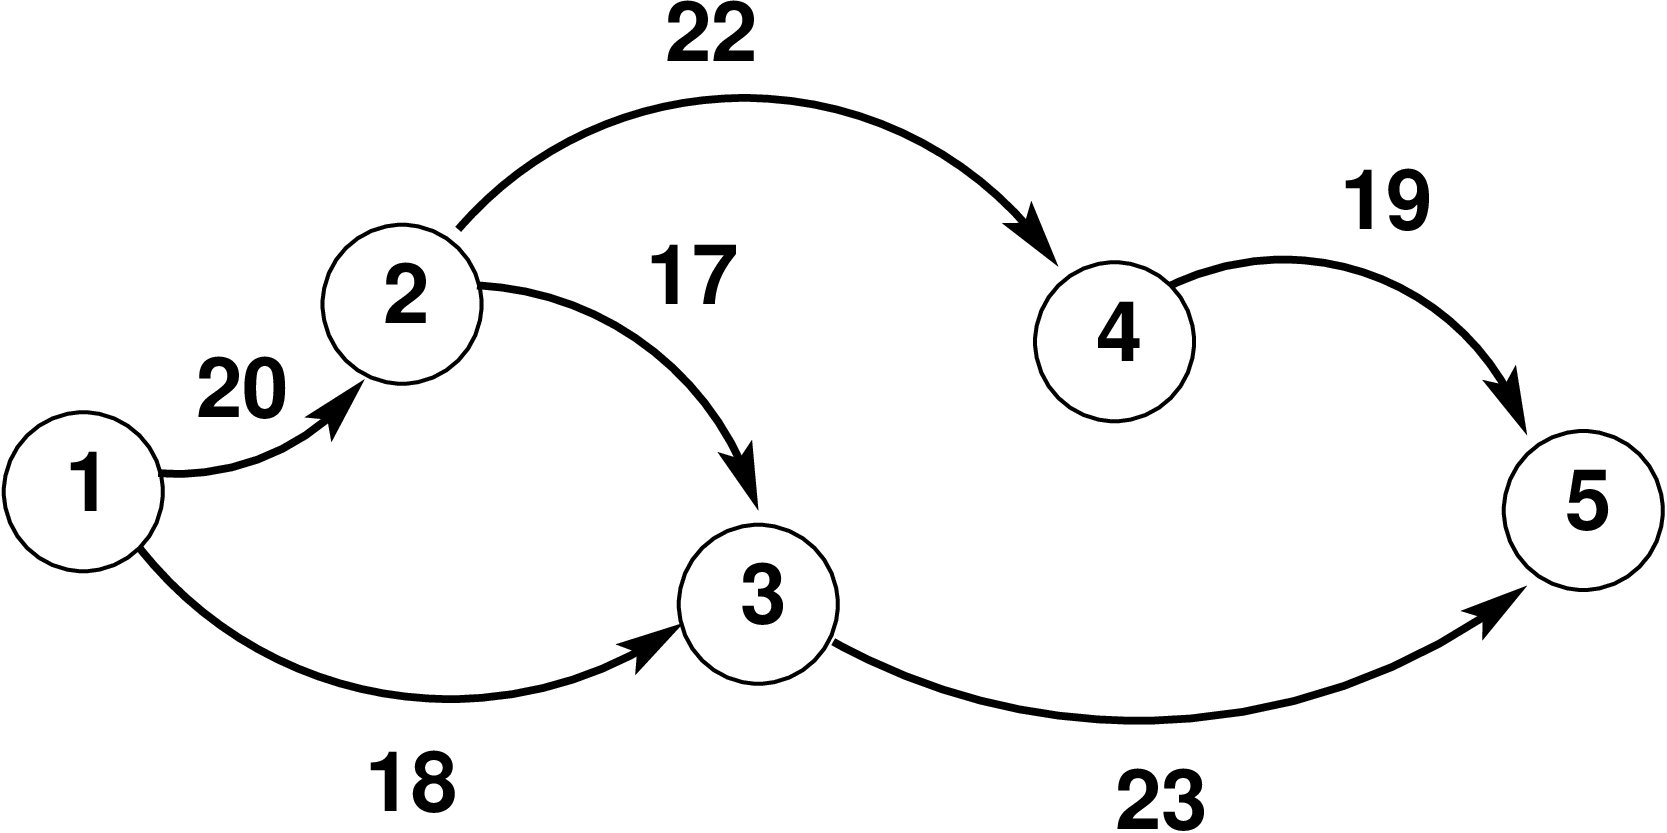
\includegraphics[width=7cm]{trevlig.png}
    \caption{The map in the second example. The nicest path is $1\rightarrow 3\rightarrow 5$.}
\end{figure}

\section*{Input}
The first line consists of the integers $n$ and $m$ ($2 \leq n \leq 10^5$, $1 \leq m \leq 2\cdot 10^5$), the number of places and the number of path segments.

Each of the following $m$ lines describe a path segment and consists of the three integers $u_i$, $v_i$ and $w_i$ ($1 \leq u_i < v_i \leq n$, $1 \le w_i \le 2\cdot 10^6$),
which means that a path segment goes from place $u_i$ to place $v_i$ with a niceness factor of $w_i$.

There will never be more than one path segment connecting two places, and it's guaranteed that it's possible to get from place $1$ to place $n$.

\section*{Output}
Output a single number: the highest possible average niceness factor on a path from place $1$ to place $n$.
Your answer will be considered correct if its relative or absolute error is at most $10^{-6}$.

\section*{Scoring}
Your solution will be tested on a set of test groups, each worth a number of points.
To get the points for a test group you need to solve all test cases in the test group.

\noindent
\begin{tabular}{| l | l | p{12cm} |}
  \hline
  Group & Points & Constraints \\ \hline
  $1$   & $21$       & $2 \le n \le 10$, $1 \le m \le 20$ \\ \hline
  $2$   & $41$       & $2 \le n \le 1000$, $1 \le m \le 2000$\\ \hline
  $3$   & $28$       & No additional constraints. \\ \hline
\end{tabular}
